\chapter{Criticallink MitySOM SoC}
Altera was founded in 1983 and developed their first FPGA in 1992.\cite{althist16} The Altera Cyclone V was developed to decrease time-to-market and cost requirements, simultaneously the power consumption is decreased. Cyclone V devices are made in 28nm technology and have a core volage of 1.1V. The 10kB memory blocks have a built in soft ECC.\cite{altcycvov15}\\
The Cyclone V SoC is built up of a FPGA and a dual-core ARM Cortex HPS. Both portions are connected using a FPGA-HPS-bridge. A high-level structural block diagram of the SoC device is shown in figure \ref{fig:alterasocblocks}. The HPS is connectable to a wide set of peripherals and supports symmetric and asymmetric multiprocessing.
\begin{figure}[htbp]
\begin{center}
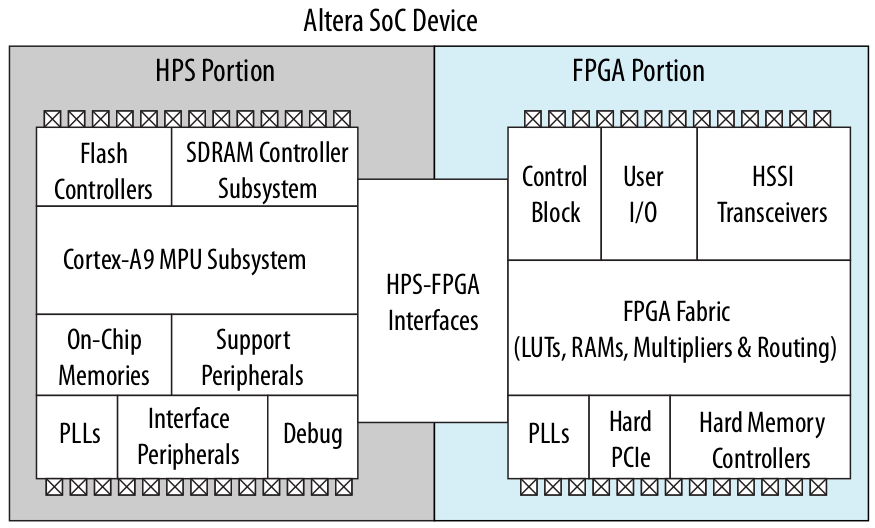
\includegraphics[width=10cm,keepaspectratio=true]{bilder/png/AlteraSoC}
\caption{Block diagram of an Altera Cyclone V SoC\cite[chapter 1]{AlteraHPS15}}
\label{fig:alterasocblocks}
\end{center}
\end{figure}
\section{FPGA}


\section{HPS}
\begin{figure}[htbp]
\begin{center}
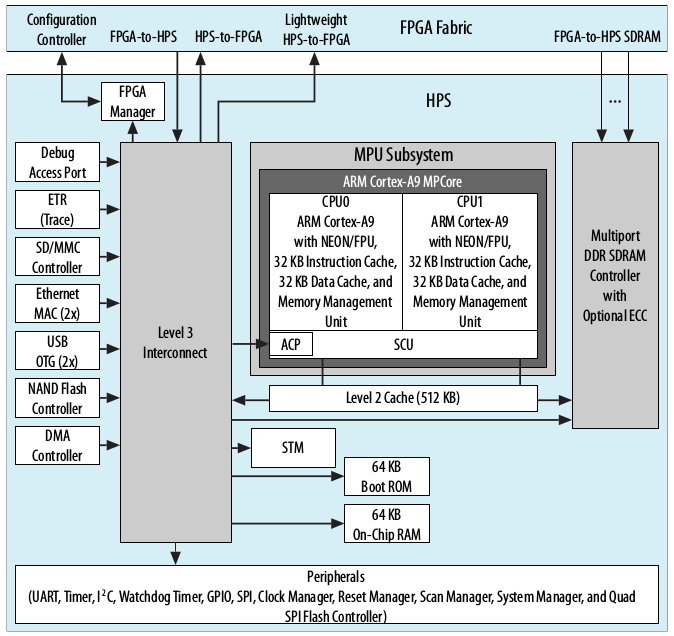
\includegraphics[width=15cm,keepaspectratio=true]{bilder/png/AlteraHPSneu}
\caption{Block diagram of an Altera Cyclone V HPSneu\cite{altcycvov15}}
\label{fig:alterahpsblocksneu}
\end{center}
\end{figure}
\begin{figure}[htbp]
\begin{center}
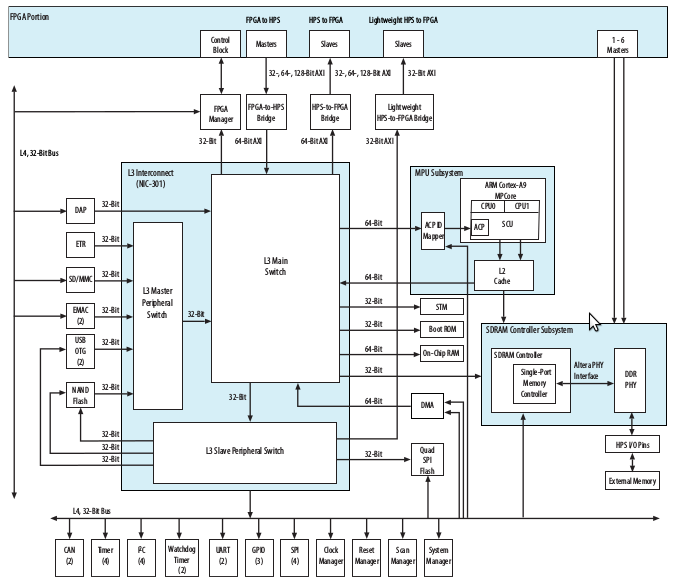
\includegraphics[width=15cm,keepaspectratio=true]{bilder/png/AlteraHPS}
\caption{Block diagram of an Altera Cyclone V HPS\cite[chapter 1]{AlteraHPS15}}
\label{fig:alterahpsblocks}
\end{center}
\end{figure}
%MPU subsystem
\subsection{MPU subsystem}
The HPS consists mainly of a 32-bit dual-core ARM Cortex A9 microprocessor, with 32kB instruction cache and 32kB data cache for each processor core. The two caches are independent and therefore simultaneous loading of instructions and data. Each cache supports parity checking. The latency of loading data depends on the availability of the data. In case of data and instruction are available in the L1 cache the hit takes 1 clock cycle, if it is available in the L2 cache the best case is 6 cycles. If the data is not available in a cache the latency vary depending on other operations. For this a so called preload engine (PLE) is implemented. This hardware block allows the L2 cache to preload different memory regions defined by software control. Furthermore the endianess of the system can be configured.\\
In a shared system with multi-processing possibilities and a single data source a hardware block to ensure coherency between processor cores and to ensure data consistency is needed. For this reason a snoop control unit (SCU) is implemented. This unit manages the data traffic for all Cortex A9 processor cores and the memory system including the L2 cache. In case of a SMP configuration also the data caches are maintained. Coherency of the instruction caches is not maintained in the SMP nor in the AMP configuration. Implementation details of the SCU can be found in \cite[chapter 9]{AlteraHPS15}.\\
For an efficient calculation of floating point operations a FPU with full support of IEEE-754 half, full and double precision data is available, as well as convertion functionality between integer and floating point data types. For fast calculation of signal processing applications such as video and audio processing an additional block called multimedia processing engine (MPE) is implemented. The MPE supports SIMD processing. The principle of SIMD is shown in figure \ref{fig:alterahpssimd}.
\begin{figure}[htbp]
\begin{center}
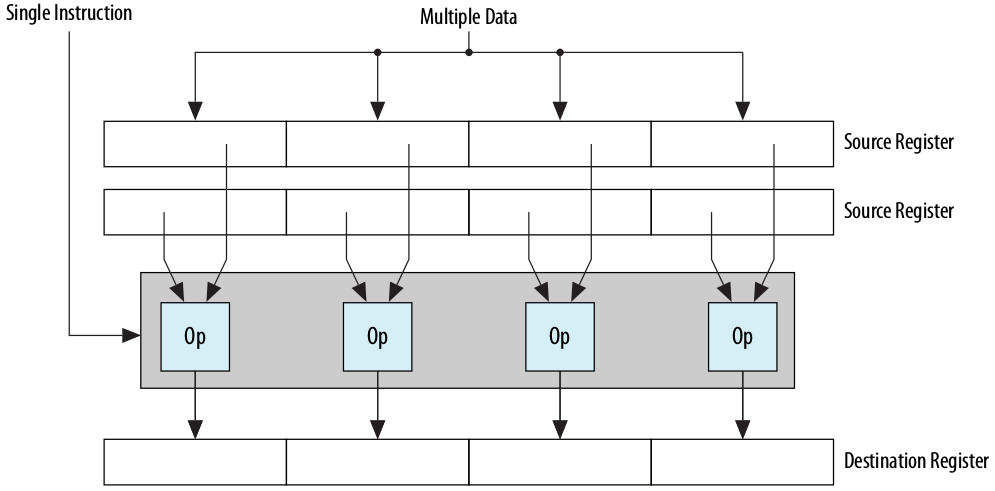
\includegraphics[width=12cm,keepaspectratio=true]{bilder/png/SIMD}
\caption{Principle of SIMD processing\cite[chapter 9]{AlteraHPS15}}
\label{fig:alterahpssimd}
\end{center}
\end{figure}
%SDRAM Controller Subsystem
\subsection{SDRAM controller subsystem}
The HPS SDRAM controller subsystem is used to access an external SDRAM memory with size of up to 4 GB for following elements and interfaces:
\begin{itemize}
\item the MPU subsystem: dedicated 64-bit AXI interface.
\item the FPGA portion: The interface consists of 64-bit read data ports, 64-bit write data ports and command ports to build up three AXI interfaces or six Avalon-MM interfaces in total.
\item the L3 interconnect: dedicated 32-bit AXI interface.
\end{itemize}
Therefore this subsystem provides an interface between the HPS and the FPGA portion. The SDRAM controller can be subdivided in a MPFE and a single-port controller. While the single-port controller communicates with each external memory device, the MPFE provides several interfaces to the single-port controller through different FIFOs. As external memories DDR2, DDR3 and LPDDR2 devices can be used. Implementation details of the SDRAM controller subsystem can be found in \cite[chapter 11]{AlteraHPS15}.
%SD/MMC-Controller
\subsection{SD/MMC-Controller}
As the internal memory of the Altera SoC has a very limited On-Chip memory, the storage of preloaders and operating systems for the HPS on external memory devices is very useful. For this reason a SD/MMC controller for using SD and MMC flash cards as well as CE-ATA hard drives is implemented. The HPS has access to this controller with a 32-bit bus via the L3 interconnect. The SD/MMC-controller supports voltage levels of 3V and, if it is supported by the card after power up, 1.8V. It has to be noted that that kind of voltage switching is not supported by the controller itself but can be done using GPIO. Implementation details can be found in \cite[chapter 14]{AlteraHPS15}.
%System interconnect
\subsection{System interconnect}
The data exchange between different hardware blocks of the HPS is done via the interconnect system, consisting of the L3 main interconnect and the L4 bus system. Furthermore the L3 system has 3 major parts:
\begin{itemize}
\item L3 interconnect, with a data width of 64 bit. It is used to connect master blocks to slaves like SDRAM controller subsystem, on-chip memories or the FPGA manager.
\item L3 master peripheral switch. This part has a data witdh of 32 bit and is used for memory-mastering peripherals.
\item L3 slave peripheral switch. Masters of the master peripheral switch and the interconnect use this block for interconnect. The data width is 32 bit. Furthermore the L3 slave peripheral switch has 5 different L4 buses.
\end{itemize}
While the master peripheral as well as the slave peripheral switch are fully connected crossbars, the L3 interconnect is partially connected. Therefore a data exchange is only possible for predefined block combinations. Those can be found in \cite[chapter 7]{AlteraHPS15}.
%Clock manager
\subsection{Clock Manager}
In the HPS different clocks organized in clock groups are used. Every clock is derived of the two main clocks \texttt{HPS\_CLK1} and \texttt{HPS\_CLK2} of the system. The clock generation of the HPS is done by the clock manager hardware block, shown in figure \ref{fig:hpsclockmanager}. 
\begin{figure}[htbp]
\begin{center}
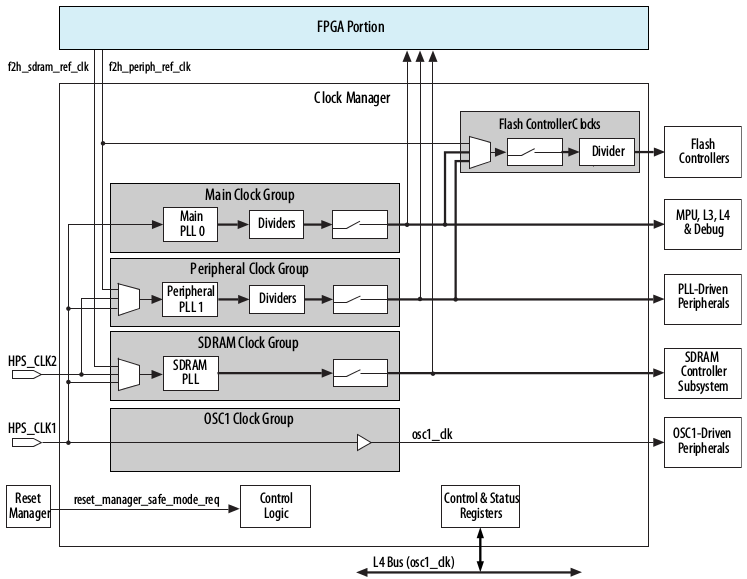
\includegraphics[width=15cm,keepaspectratio=true]{bilder/png/hpsclockmanager}
\caption{Clock generation of an Altera Cyclone V HPS\cite{altcycvov15}}
\label{fig:hpsclockmanager}
\end{center}
\end{figure}
A derivation of the different clocks is done using a PLL, where the frequency is set with a VCO. Dividers are used to lower the generated frequency. For generating clocks three PLLs are available. The clock manager contains 4 different clock groups:
\begin{itemize}
\item OSC1 clock group\\
This clock group has only one clock which is not divided and directly taken from the \texttt{HPS\_CLK1} as input for a PLL. It is used for OSC1-driven peripherals.
\item main clock group\\
The PLL input of this group is derived of the \texttt{HPS\_CLK1}. It contains 5 dividers to generate different clocks for the MPU, SD/MMC-controller or, among others, the system interconnect.
\item peripheral clock group\\
This group is used for clocking interfaces like USB, CAN and GPIO. The PLL can be sourced either from \texttt{HPS\_CLK1}, \texttt{HPS\_CLK2} or the \texttt{f2h\_periph\_ref\_clk} provided by the FPGA. The peripheral clock group has 5 dividers to provide 5 different clocks.
\item SDRAM clock group\\
The SDRAM clock group can use the  \texttt{HPS\_CLK1}, \texttt{HPS\_CLK2} or the \texttt{f2h\_sdram\_ref\_clk} clock provided by the FPGA for the SDRAM PLL.
\end{itemize}
A detailed description of the different clocks generated in the clock groups can be found in \cite[chapter 2]{AlteraHPS15}.
\subsubsection{Considerations on the used PLL}
The VCOs of the used PLLs have frequency stability up to +/- 20 percent of the used frequency and does not lose the PLL locking within this range. So when there is a need for changing the frequency more than 20 percent a slow ramp up or down of the VCO is a possibility to change frequency without loosing the lock. An other possibility, when e.g. lowering the frequency to the half is to decrease the frequency by 20 percent for three times and divide it by 2.4 percent in a last step.
%System manager
\subsection{System Manager}
The system manager connects modules for system level functions like DMA or the SD/MMC-controller. Furthermore it contains CSRs to monitor and control functions by software access. The system manager also contains information about boot configurations and defines which bootROM-code to execute. Detailed descriptions of how the system manager works and how the different controllers of the system manager are defined can be found in \cite[chapter 5]{AlteraHPS15}.
%FPGA manager
\subsection{FPGA Manager}
This module of the HPS is used to manage and configure the FPGA of the SoC. For this 32 general-purpose input as well as 32 general-purpose output signals to the FPGA are available. Handshaking is also done using this block when booting the HPS from the FPGA portion. When the FPGA is in user mode it offers following registers for low latency communication between FPGA and HPS:
\begin{itemize}
\item \texttt{gpi}: general-purpose input register. The 32 input signals from the FPGA are read from this register.
\item \texttt{gpo}: general-purpose output register. Output signals to the FPGA are written to this register.
\item \texttt{misci}: boot handshaking input register. Those 2 signals are used by the bootROM code to determine if the preloader image stored in the FPGA should be used for the boot process.
\end{itemize}
For more information about the implementation of the FPGA manager see \cite[chapter 5]{AlteraHPS15}.
%FPGA-HPS-Bridge
\subsection{HPS-FPGA-bridges}


\section{Interfaces}
\subsection{UART}
UART is a transmission protocol which was developed in the 1960s. UART is highly flexible in the sense that voltages, timing, error checking and flow control can be configured as the application needs. The commonly supported baud rates of UART are 600-921600 baud/s. As the history of UART is quite long some different physical layer standards have been developed, such as RS232C or RS485. Due to this long development history also quite some radiation hardened devices exist, like the Aeroflex DRS4485.\cite{aeroflex14}
\subsection{GPIO}
A GPIO is a digital interface which is made of pins with no dedicated usage. It is possible to configure them flexible during runtime to act as input or output.
\begin{itemize}
\item When the pin is configured as input it can read data from a digital circuit
\item A binary signal can be sent to a digital circuit when the pin is configured as output.
\end{itemize}
GPIO-pins are available on most SoC and FPGA-devices, in some cases it is possible to configure every pin with no dedicated usage as GPIO-pin.\cite{kernelgpio15}
\subsection{I$^2$C}
The I$^2$C-bus was intentionally developed by Philips in the early 1980s to exchange information between ICs located on the same board. This bus is designed for synchronous transmission and is built up of ground, data and clock line. As advantage of this protocol the clock reconstruction possibilities at the receiver has to be mentioned. Furthermore an arbitrary protocol guarantees that only one master exists at one time.\cite{Wue06} I$^2$C defines communication modes as follows:
\begin{table}
\begin{center}
\begin{tabular}{|c||c|c|}
\hline
mode & maximum transmission speed & direction\\
\hline\hline
standard mode & 100 kbit/s & bidirectional\\
\hline
full speed & 400 kbit/s & bidirectional\\
\hline
fast mode & 1 Mbit/s & bidirectional\\
\hline
high speed mode & 3.2 Mbit/s & bidirectional\\
\hline
ultra fast mode (UFm) & 5 Mbit/s & unidirectional\\
\hline
\end{tabular}
\caption{Speed grades of I$^2$C-transmissions\cite{I2Cspeed}}
\label{tab:rsstates}
\end{center}
\end{table}
As the I$^2$C-bus is inteded to exchange data between ICs the packet size is small. This leads to the fact that high accuracy of the clock is not needed for most applications.\cite{I2Cspeed} Intentionally the I$^2$C-bus was designed for 5V reference voltage. With the release of the specification I$^2$C-2.0 the bus got also the possibility to operate with 2V references.\cite{I2Cvoltage}
More information can be found in the I$^2$C-specification in \cite{I2Cspec}.
\subsection{CAN}
The CAN-bus was developed by Bosch in the early 1980s as serial communication protocol for motorized vehicles. In 1994 it became an international standard ISO 11898. The protocol is able to handle bitrates up to 1 Mbit/s and has multi-master capability. That means that different bus members can have master state at different times. CAN is able to handle reference voltages of 5V and 3.3V.\cite{Corrig2008} The CAN-bus uses two signaling lines for communications. As CAN is designed as real time control protocol with a high level of security, it has some important features beside others\cite{boschcan91}:
\begin{itemize}
\item message priorization
\item guaranteed latency times
\item different error detection capabilities
\item autonomous switching off of defect nodes
\end{itemize}
The specification of CAN can be found in \cite{boschcan91}, an even more detailed description in \cite{nxpcan98}.
\section{booting}
For booting three different configuration options are possible:\cite[chapter A]{AlteraHPS15}
\begin{itemize}
\item The HPS preloader and the FPGA configuration are independent. In this case the FPGA configuration image is loaded from an external source, the HPS preloader is also located externally.
\item The HPS boots and the FPGA is configured after this by the HPS. The HPS preloader is loaded from an external memory. After the boot of the HPS the FPGA is reset and a configuration image from a flash memory or a communication interface is loaded by the HPS to the FPGA.
\item The FPGA is configured and the HPS boots from the FPGA portion. For this the FPGA configuration image is loaded from an external source. The FPGA is configured and contains a preloader image for the HPS. When using this initialization option the HPS should not be released from reset state until the FPGA configuration is completed. After the HPS release the HPS preloader image is executed by the BootROM over the FPGA-HPS-bridge.
\end{itemize}
The boot flow is shown in figure \ref{fig:bootstages}.
\begin{figure}[htbp]
\begin{center}
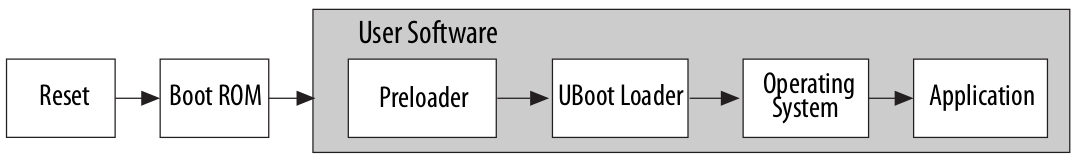
\includegraphics[width=13cm,keepaspectratio=true]{bilder/png/bootstages}
\caption{Boot steps of an Altera Cyclone V SoC\cite[chapter A]{AlteraHPS15}}
\label{fig:bootstages}
\end{center}
\end{figure}
\subsection{Reset}
\begin{itemize}
\item cold reset\\
In this case all registers are initialized and the HPS starts executing the BootROM code located at the reset exception address. A cold reset is done whenever the device is booted after a full shutdown.
\item warm reset\\
In case of a warm reset some register contents are preserved. In addition the device has the ability to execute a preloader located in the on-chip RAM.
\end{itemize}
\subsection{Boot-ROM}
The boot-ROM is located in the on-chip ROM and performs all actions needed for a basic initialization of the system. It determines the boot source, selected with the \texttt{BSEL}-pins and configures the main PLL clock rate using the \texttt{CSEL}-pins. Furthermore the flash controller is set to default settings. After initialization the boot-ROM jumps to the preloader. Depending on the location of the preloader, the first 4kB of the on-chip RAM are used. When the preloader image is located on a flash device, this memory is reserved as working space for the HPS, otherwise it can be used for user purposes. It has to be noted, that the Boot-ROM is always executed on CPU core 0. After the Boot-ROM has switched the control to the user software (the preloader) the access to the Boot-ROM is disabled.
\subsubsection{booting from SD/MMC flash devices}
If the preloader image is stored on a flash device as shown in figure \ref{fig:sdboot}, the first 512 byte of the storage are used as MBR where the start addresses and sizes of the boot images on the device are stored. The images themselfes are stored in a raw partition with no file system (shown as partition A2). As the on-chip RAM-size is limited to 64kB and 4kB are used as working memory (stack, ...) the preloader image has to have a maximum size of 60kB. In case of a failure of the flash device, the Boot-ROM checks the FPGA portion for a bootable fallback image. 
\begin{figure}[htbp]
\begin{center}
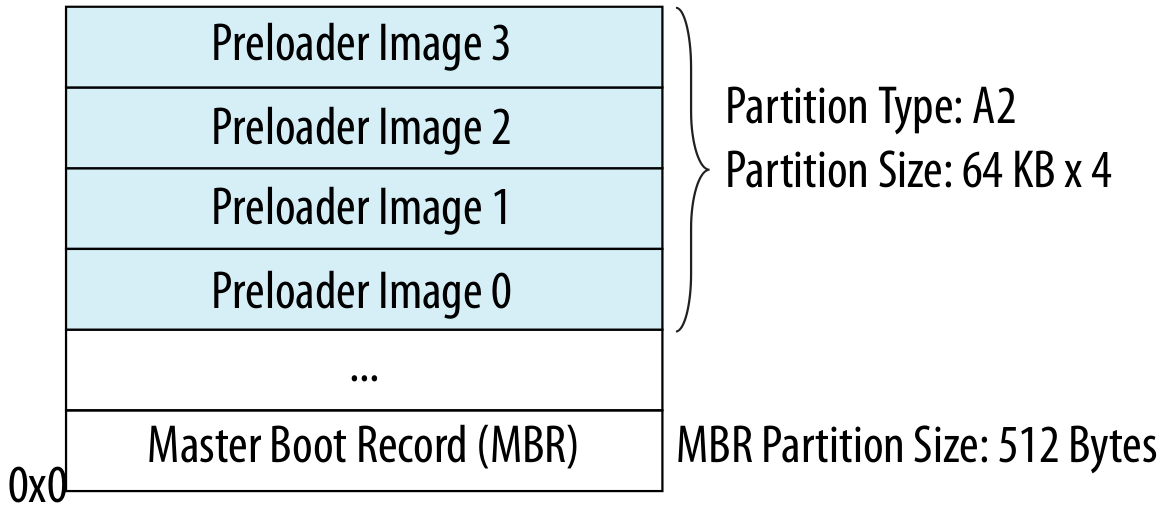
\includegraphics[width=8cm,keepaspectratio=true]{bilder/png/sdboot}
\caption{SD/MMC boot image layouts\cite[chapter A]{AlteraHPS15}}
\label{fig:sdboot}
\end{center}
\end{figure}
\subsection{Preloader}
The preloader is the first stage of the user software. Therefore the functionality of the preloader image is given by the user. Typical functions include the initialization of interfaces for booting the next software stage and the SDRAM interface. Furthermore the I/O-pins can be configured. The next software stage can be loaded from any interface available to the HPS and, after initialization of the SDRAM, is not limited to 60kB as it is for the on-chip ROM.
\subsection{UBoot-Loader}
UBoot is an universal bootloader for a variety of devices, especially made for embedded systems. It was invented by DENX in 1999 and available under the GPL. UBoot can be configured using a command line interface, the configuration can be safed to flash devices. Typically the UBoot-loader sets up the device tree, loads the operating system kernel and hands over the user software control to the kernel.
\subsection{Operating System}